\documentclass[oneside]{VUMIFPSkursinis}
\usepackage{algorithmicx}
\usepackage{algorithm}
\usepackage{algpseudocode}
\usepackage{amsfonts}
\usepackage{float}
\usepackage{amsmath}
\usepackage{bm}
\usepackage{caption}
\usepackage{color}
\usepackage{float}
\usepackage{graphicx}
\usepackage{listings}
\usepackage{subfig}
\usepackage{ltablex}
\usepackage{longtable}
\usepackage{wrapfig}
\usepackage{subfig}
\usepackage{pbox}
\renewcommand{\labelenumii}{\theenumii}
\renewcommand{\theenumii}{\theenumi.\arabic{enumii}.}
\renewcommand{\labelenumiii}{\theenumiii}
\renewcommand{\theenumiii}{\theenumii\arabic{enumiii}.}
\newcolumntype{P}[1]{>{\centering\arraybackslash}p{#1}}
\usepackage[%
	colorlinks=true,
	linkcolor=black
]{hyperref}
\university{Vilniaus universitetas}
\faculty{Matematikos ir informatikos fakultetas}
\department{Programų sistemų katedra}
\papertype{Žmogaus ir kompiuterio sąsaja laboratorinis darbas V}
\title{Prototipo testavimas}
\titleineng{Aludarystės internetinė parduotuvė}
\status{3 kurso studentai}
\author{Greta Pyrantaitė}
\secondauthor{Matas Savickis}
\thirdauthor{Andrius Bentkus}

\supervisor{Kristina Lapin, Doc., Dr.}
\date{Vilnius – \the\year}

\bibliography{bibliografija}

\begin{document}
\maketitle

\sectionnonum{Anotacija}
Šiuo darbu siekiame įvertinti savo detaliojo maketo panaudojamumą apklausiant potencialius sistemos naudotojus. Šiame darbe pateiksime ataskaitą apie tai, kaip vartotojai įvertino sistemą, kaip sekėsi atlikti užduotis ir kokius pakeitimus siūlė įgyvendinti.

\begin{itemize}
	\item{Greta Pyrantaitė - greta.pyrantaite@gmail.com}
	\item{Matas Savickis - savickis.matas@gmail.com}
	\item{Andrius Bentkus - andrius.bentkus@gmail.com}
\end{itemize}

\tableofcontents


\sectionnonum{Santrauka}
\sectionnonum{Įvadas}
	\subsectionnonum{Prototipas}
		Prototipas demonstruoja alaus virimo reikmenų internetinės parduotuvės įgyvendinimą. Prototipas kurtas atsižvelgiant į paskaitose pateiktą teorinę medžiagą apie stiliaus ir panaudojamumo kompoziciją. Stengtasi visoje programoje išlaikyti vienodą, pastovų ir minimalistinį stilių. Įgyvendinta vartotojo(pirkėjo) ir administratoriaus(pardavėjo) vartotojo sąsaja. Prototipas kurtas naudojant Axure prototipavimo programą, apie šios programos naudojimą sužinojome iš dėstytojos pateikto vaizdo įrašo.
	\subsectionnonum{Programų sistemos ilgasis pavadinimas}
		Alaus gamybos įrangos ir ingredientų pirkimo sistema.
	\subsectionnonum{Programų sistemos trumpasis pavadinimas}
		Aludarystės internetinė parduotuvė.
	\subsectionnonum{Dalykinė sritis}
		Elektroninė parduotuvė skirta aludariams.
	\subsectionnonum{Probleminė sritis}
		Sistema turi suteikt galimybę nusipirkti alaus gamybai reikalingus ingredientus ir įrangą bei gauti visą reikalingą informaciją apie ingredientų ir įrangos specifikacijas.
		Sistema taip pat turi vartotojui pateikti informaciją apie alaus gamybos procesą panaudojant nusipirktus ingredientus ir įrangą.
	\subsectionnonum{Naudotojai}
		\begin{itemize}
			\item{Pirkėjas(aludaris) - pirkėjas turi galėti užsisakyti alaus gamybos ingridientus ir įrangą bei gauti reikalingą specifikaciją norint naudotis preke.
				Pirkėjui turi užtekti mokyklinio informatikos kurso žinių ir bendro supratimo, kaip naviguotis internetinėse svetainėse.}
			\item{Pardavėjas - pardavėjui sistema turi suteikti informaciją apie užsakymus, jų apmokėjimus ir panašią svarbią informaciją.
				Sistema pardavėjui taip pat turi suteikti galimybę pridėti arba išimti prekes iš internetinės parduotuvės.
				Pardavėjui taip pat turi užtekti mokyklinio lygio informatikos žinių ir bendrų žinių naviguotis interneto svetainėse.}
		\end{itemize}
	\subsectionnonum{Naudoti dokumentai}
		Kristina Lapin - Žmogaus ir kompiuterio sąveikos paskaitų skaidrės, laboratorinių darbų aprašymai.
	

\section{Testavimo aprašas}
	\subsection{Testuojamos užduotys}
		\begin{enumerate}
			\item{Susirasti instukciją, kaip pasigaminti alaus.}
			\item{Instrukcijos ekrane užsisakyti visas prekes.}
			\item{Instrukcijos ekrane pasirinkti kelias norimas prekes iš sąrašo.}
			\item{Peržiūrėti krepšelio turinį.}
			\item{Ištrinti prekę iš krepšelio.}
			\item{Pakeisti prekės kiekį krepšelyje.}
			\item{Atsiskaityti už prekes.}
			\item{Surasti apynius granulėmis.}
			\item{Įdėti 10 gramų apynių su didžiausiu rūgštingumu į krepšelį.}
			\item{Surūšiuoti prekių sąrašą pagal pavadinimą.}
			\item{Pardavėjo panelėje peržiūrėti Petro Petraičio užsakymą.}
			\item{Pakeisti užsakymo būseną.}
			\item{Peržiūrėti prekių sąrašą.}
			\item{Peržiūrėti fermentavimo kibiro aprašymą.}
			\item{Pakeisti prekės aprašą.}
			\item{Išimti fermentavimo kibirą iš prekybos.}
		\end{enumerate}
		Matuosime, kiek klaidų vartotojas padarė prieš atlikdamas užduotį, kiek laiko užtruko sėkmingai įvykdyti užduotį ir kiek kartų vartotojas prašė pagalbos vykdant užduotį.
	\subsection{Metodas}
		Stebėjimai testuojant su naudotojais. Vartotojai užduotis atlieka tyloje ir ekspertas tarpais įsterpia pasiteirauti nuomonės, ką jie daro. Testavimo pradžioje vartotojui pateiksime klausimyną išsiaiškinti vartotojo charakteristikom, tada vartotojui pateiksime internetinę sąsają. Iš užduočių sąrašo prašysime vartotojo vykdyti užduotis po vieną ir stebėsime vartotojo sėkmę. Vartotojas bet kuriuo metu galės prašyti pagalbos. 
	\subsection{Aplinka}
		Testavimas buvo vykdomas nuotoliniu būdu naudojanti Skype bendravimo aplikaciją.
		Vartotojo ekranas ir pelės judesiai buvo stebimi panaudojamumo ekspertų(mūsų).
		Vartotojas naudojosi nešiojamu kompiuteriu, modernia internetine naršykle ir pele.
	\subsection{Dalyviai}
\begin{center}
    \begin{tabular}{ |p{1cm} | p{2cm} | p{4cm} | p{4cm} | p{4cm} |}
    \hline
	ID&Amžius&Profesija&IT raštingumas&Susidomėjimas alaus gamyba\\ \hline
	1&50&Namų šeimininkė&Prastas&Nesusidomėjusi \\ \hline
	2&15&Moksleivė&Geras&Susidomėjusi \\ \hline
	3&22&Studentas&Puikus&Susidomėjęs \\ \hline
	4&47&Darbuotoja&Geras&Nesusidomėjusi \\ \hline
	5&49&Darbuotojas&Geras&Susidomėjęs \\ \hline
	6&23&Darbuotoja&Puikus&Susidomėjus \\ \hline
	7&61&Mokslinių žuralnų redaktorė&Pradžiamokslis&Nesusidomėjusi \\ \hline
   \hline
    \end{tabular}
\end{center}



\section{Testavimo rezultatai}
	\subsection{Užduočių vykdymo rezultatai}

	\begin{figure}[ht]
			\centering
			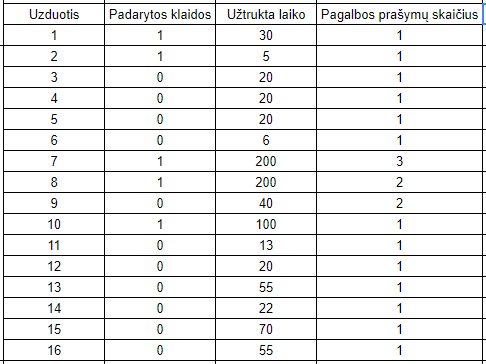
\includegraphics[width=15cm,height=60cm,keepaspectratio]{1.png}
			\caption{ Vartotojas ID: 1}
	\end{figure}

\pagebreak

	\begin{figure}[ht]
			\centering
			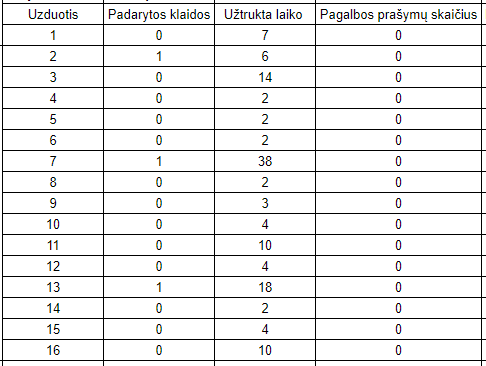
\includegraphics[width=15cm,height=60cm,keepaspectratio]{2.png}
			\caption{ Vartotojas ID: 2}
	\end{figure}
\pagebreak

	\begin{figure}[ht]
			\centering
			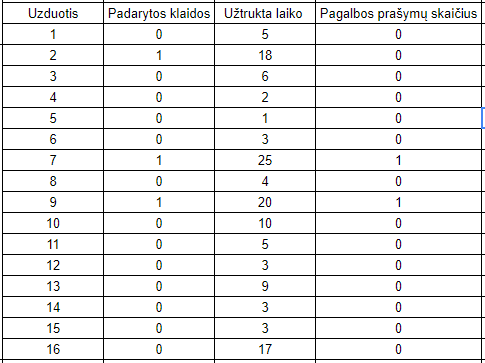
\includegraphics[width=15cm,height=60cm,keepaspectratio]{3.png}
			\caption{ Vartotojas ID: 3}
	\end{figure}
\pagebreak
	
	\begin{figure}[ht]
			\centering
			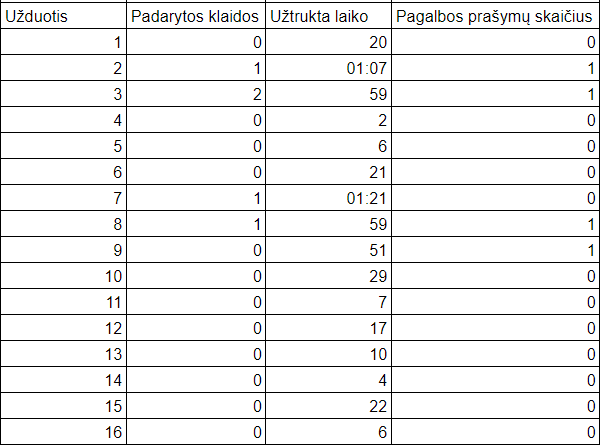
\includegraphics[width=15cm,height=60cm,keepaspectratio]{4.png}
			\caption{ Vartotojas ID: 4}
	\end{figure}
\pagebreak

	\begin{figure}[ht]
			\centering
			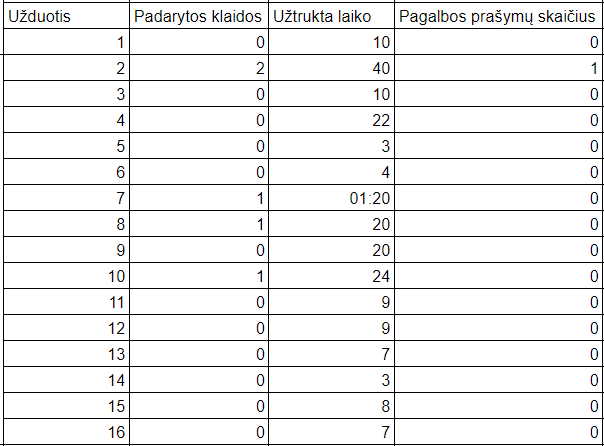
\includegraphics[width=15cm,height=60cm,keepaspectratio]{5.png}
			\caption{ Vartotojas ID: 5}
	\end{figure}
\pagebreak

	\begin{figure}[ht]
			\centering
			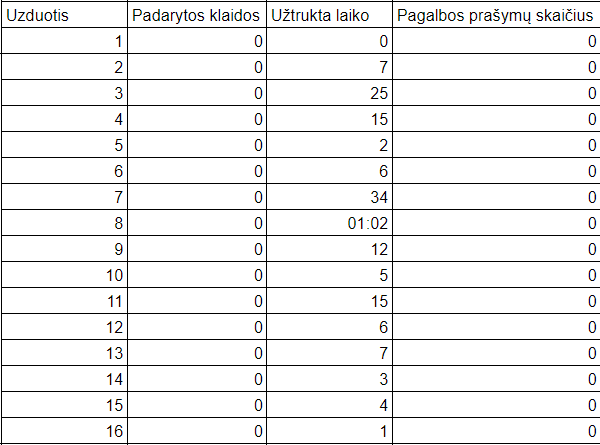
\includegraphics[width=15cm,height=60cm,keepaspectratio]{6.png}
			\caption{ Vartotojas ID: 6}
	\end{figure}
\pagebreak

	\begin{figure}[ht]
			\centering
			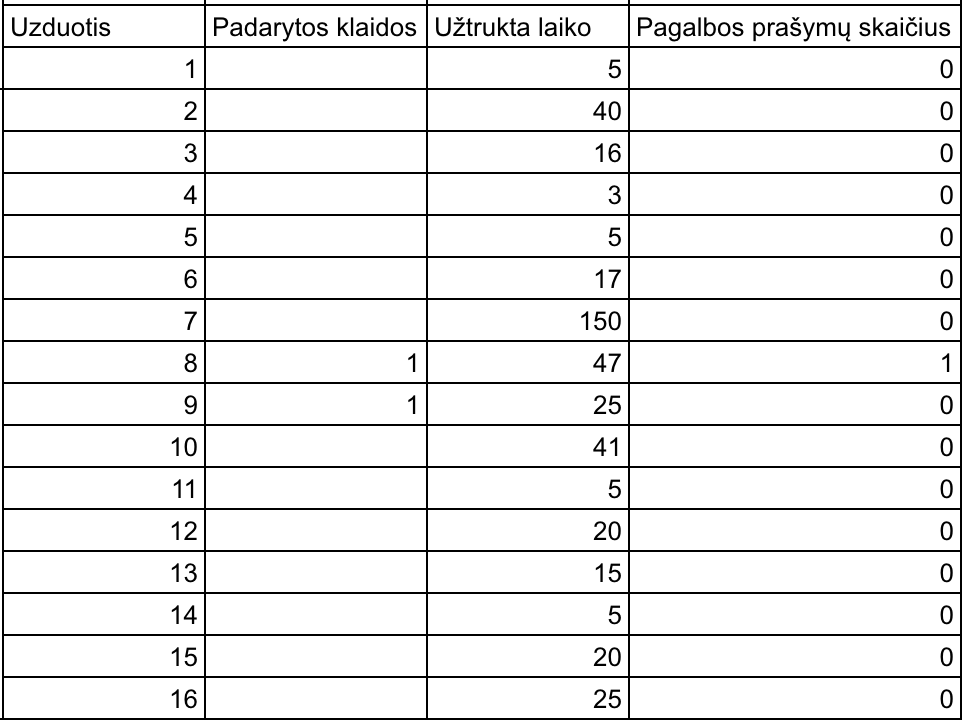
\includegraphics[width=15cm,height=60cm,keepaspectratio]{7.png}
			\caption{ Vartotojas ID: 7}
	\end{figure}

	\subsection{Dalyvių komentarai}
\begin{center}
    \begin{tabular}{ |p{3cm}| p{12cm} |}
    \hline
	Užduoties Nr.&Komentarai\\ \hline
	2&Kodėl šitas mygtukas taip žemai, nesimato nieko.\\ \hline
	3&Galima aiškiau parašyti ''pasirinkti''\\ \hline
	4&Geriau parašyti ''krepšelis''\\ \hline
	7&O tai kodėl aš galiu nusipirkti neįvedus adreso? Neaiškus eiliškumas.\\ \hline
	8&Neaišku, kokiam kiekiui kaina\\ \hline
	10&Nepatogioj vietoj rūšiavimo mygtukas, lengviau būtų jeigu jis būtų virš prekių sąrašo\\ \hline
	16&Tai kad prekių saraše nėra mygtuko ištrinti čia jokio.\\ \hline
	2&Mygtukas įdėti visom prekėm yra nereikalingas, niekas jo nenaudoja.\\ \hline
	7&Nesuprato kad reikia atsikleisti pirmą elementa, tam kad prisiloginti. Nesuprato kaip tęsti toliau.\\ \hline
	9&Trūksta matų vienetų, šiauo atvėju gramų.\\ \hline
	9&Įdedant į krepšelį neaišku kiek įdėta, nes neparodo.\\ \hline
	16&Neaišku ką peržiūrėti, pavadinimas "peržiūrėti" yra neaiškus. \\ \hline
    \end{tabular}
\end{center}

\subsection{Apibendrinimas}

\begin{center}
    \begin{tabular}{ |p{3cm}| p{3cm} |p{3cm}|p{3cm}|p{3cm}|}
\hline
Užduoties Nr.&Sėkmingai įvykdė&Vykdymo laiko vidurkis (s)&Kiek kartų kreiptąsi pagalbos&Padarytos klaidos\\ \hline
	1  & 100\% & 11 & 1 & 1 \\ \hline
	2  & 100\% & 26 & 3 & 6 \\ \hline
	3  & 100\% & 21 & 2 & 2 \\ \hline
	4  & 100\% &  9 & 1 & 0 \\ \hline
	5  & 100\% &  6 & 1 & 0 \\ \hline
	6  & 100\% &  8 & 1 & 0 \\ \hline
	7  & 100\% & 86 & 4 & 5 \\ \hline
	8  & 100\% & 56 & 4 & 4 \\ \hline
	9  & 100\% & 24 & 4 & 2 \\ \hline
	10 & 100\% & 27 & 1 & 2 \\ \hline
	11 & 100\% &  9 & 1 & 0 \\ \hline
	12 & 100\% & 11 & 1 & 0 \\ \hline
	13 & 100\% & 17 & 1 & 1 \\ \hline
	14 & 100\% &  6 & 1 & 0 \\ \hline
	15 & 100\% & 19 & 1 & 0 \\ \hline
	16 & 100\% & 17 & 1 & 0 \\ \hline
\end{tabular}
\end{center}	
		
\section{Rekomendacijos}
\begin{itemize}
	\item{Dažnis - iš 7 vartotojų kurie testavo maketą, kiek iš jų susidūrė su defektu}
	\item{Prioritetas - Lengvas(menkas vizualinis trukdis, kuris gali būti neištaisytas);Vidutinis(defektas, kuris įtakoja vartotojo navigaciją ar kažkaip kitaip pablogina vartotojo patirtį);Sunkus(defektas, kuris sukelia dviprasmybes sistemos navigacijoje ar kitaip sutrikdo vartotojo patirtį. Šį defekta būtina ištaisyti.)}
\end{itemize}
\begin{center}
    \begin{tabular}{ |p{2cm}| p{4cm} | p{2cm} | p{2cm} | p{5cm} |}
    \hline
	Užduoties Nr.&Defektas&Dažnis&Prioritetas&Siūlomas sprendimas\\ \hline
	2&Sunku rasti ''Pirkti viską'' mygtuką.&4&Vidutinis&Pakelti mygtuką aukščiau, kad būtų labiau matomas. \\ \hline
	4&Kartais ne iki galo aiškus krepšelio simbolis.&2&Lengvas&Parašyti šalia ''Krepšelis''. \\ \hline
	7&Neaiškus ir klaidų netikrinantis apmokėjimas.&4&Sunkus&Neleisti vartotojui toliau pildyti nepatikrinus įvestų duomenų, pateikti kitokiu formatu negu išskleidžiamu. \\ \hline
	8&Neaišku, kokiam kiekiui kaina.&4&Sunkus&Parašyti šalia kainos, kokiam kiekiui ji taikoma. \\ \hline
	10&Nepatogioj vietoj rūšiavimo pasirinkimas.&4&Lengvas&Pakelti rūšiavimą į viršų. \\ \hline
   \hline
    \end{tabular}
\end{center}
\section{Priedai}
	\subsection{Klausimynai}
	\subsubsection{Klausimynas prieš testavimą}
	\begin{enumerate}
			\item{Koks Jūsų amžius?}
			\item{Kokia Jūsų profesija?}
			\item{Koks Jūsų raštingumo IT lygis?}
			\item{Kiek esate susidomėję alaus gamyba?}
	\end{enumerate}
	\subsubsection{Klausimynas po testavimo}
	\begin{enumerate}
			\item{Kas labiausiai patiko prototipe?}
			\item{Kas labiausiai nepatiko?}
			\item{Ką labiausiai reikia keisti?}
			\item{Ar buvo lengva vykdyti užduotis?}
	\end{enumerate}
	
	\subsection{Dalyvių rezultatų lentelės}
\begin{center}
    \begin{tabular}{ |p{1cm} | p{3cm} | p{4cm} | p{4cm} | p{3cm} |}
    \hline
	ID&Kas labiausiai patiko&Kas labiausiai nepatiko&Ka reiktų pakeisti&Ar buvo lengva įvykdyti užduotis\\ \hline
	1&Niekas&Nesusigaudau niekur&Nieko&Buvo lengva(sarkastiškai) \\ \hline
	2&Aiškus puslapis ir nesunku viską surasti&Kad reikėjo užpildyti daug informacijos prieš užsisakant&Nežinau&Taip \\ \hline
	3&Gražus pagrindinis puslapis&Neaišku, kada prekė įdedama į krepšelį. Rušiavimo mygtukas nepatogioje vietoje&Perkelti rušiavimo mygtuką į viršų. Padaryti, kad būtų galima grįžti iš pardavėjo panelės į vartotojo pagrindinį langą. Padaryti, kad būtų galima naviguotis paspaudus ant duonos trupinių&Taip \\ \hline
	4&Dizainas, instrukcija.&Neaiškūs kiekiai.&Smulkmenas, aiškumą.&Visai jo. \\ \hline
	5&Kibiras.&Nuobodi programa.&Nieko.&Lengva. \\ \hline
	6&Gana suprantama.&Dizainas (spalvos, šriftas, pasenęs).&Dizainą.&Taip. \\ \hline
	7&Paprastumas&Lietuviški pavadinimai&Funkcionalumas nepilnas, reiktų iškarto rodyti prekių skaičių krepšelyje, rūšiavimo parinktis ne "vietoj", reiktų aiškiai pavadinti "prekių rūšiavimas", ropdyklę prie apinių pagrindiniam meniu yra nesuprantama, išreikti reiktų pavadinimu "apinių tipai".&Taip. \\ \hline
   \hline
    \end{tabular}
\end{center}

\end{document}
